\section{Ping}
Per quanto riguarda l'utilizzo del comando \textit{ping} l'opzione utilizzata è la \textit{-i} con i valori 0.001/0.1/0.3/0.5.\\
Come già accennato in precedenza, Snort rileva immediatamente un qualsiasi attacco basato su pacchetti ICMP, come ad esempio gli attacchi che utilizzano il comando ping (ping of death, denial of service, ...). Questo si vede facilmente dai grafici che mostrano come in tutti i casi il tempo di rilevamento da parte di Snort di un attacco ping sia immediato. Per quanto riguarda invece la durata complessiva dell'attacco si ha che, come ci si può aspettare, a parità di pacchetti inviati (100, in questi esperimenti) la durata dell'attacco aumenta al diminuire del rate di invio: inviando ad un rate di 0.001 pacchetti/secondo l'attacco termina in meno di mezzo secondo, mentre inviando ad una frequenza di 0.5 pacchetti/secondo la durata aumenta fino a quasi 50 secondi complessivi\\
Inoltre dall'analisi dei log è possibile osservare che per un rate di invio pare a 0.5 pacchetti/secondo non viene generato alcun alert del tipo \textit{``TOO MUCH PING''}, verificando che l'introduzione della nostra regola permette di stabilire una soglia oltre la quale si può ritenere dannosa la sottomissione di ping troppo frequenti.

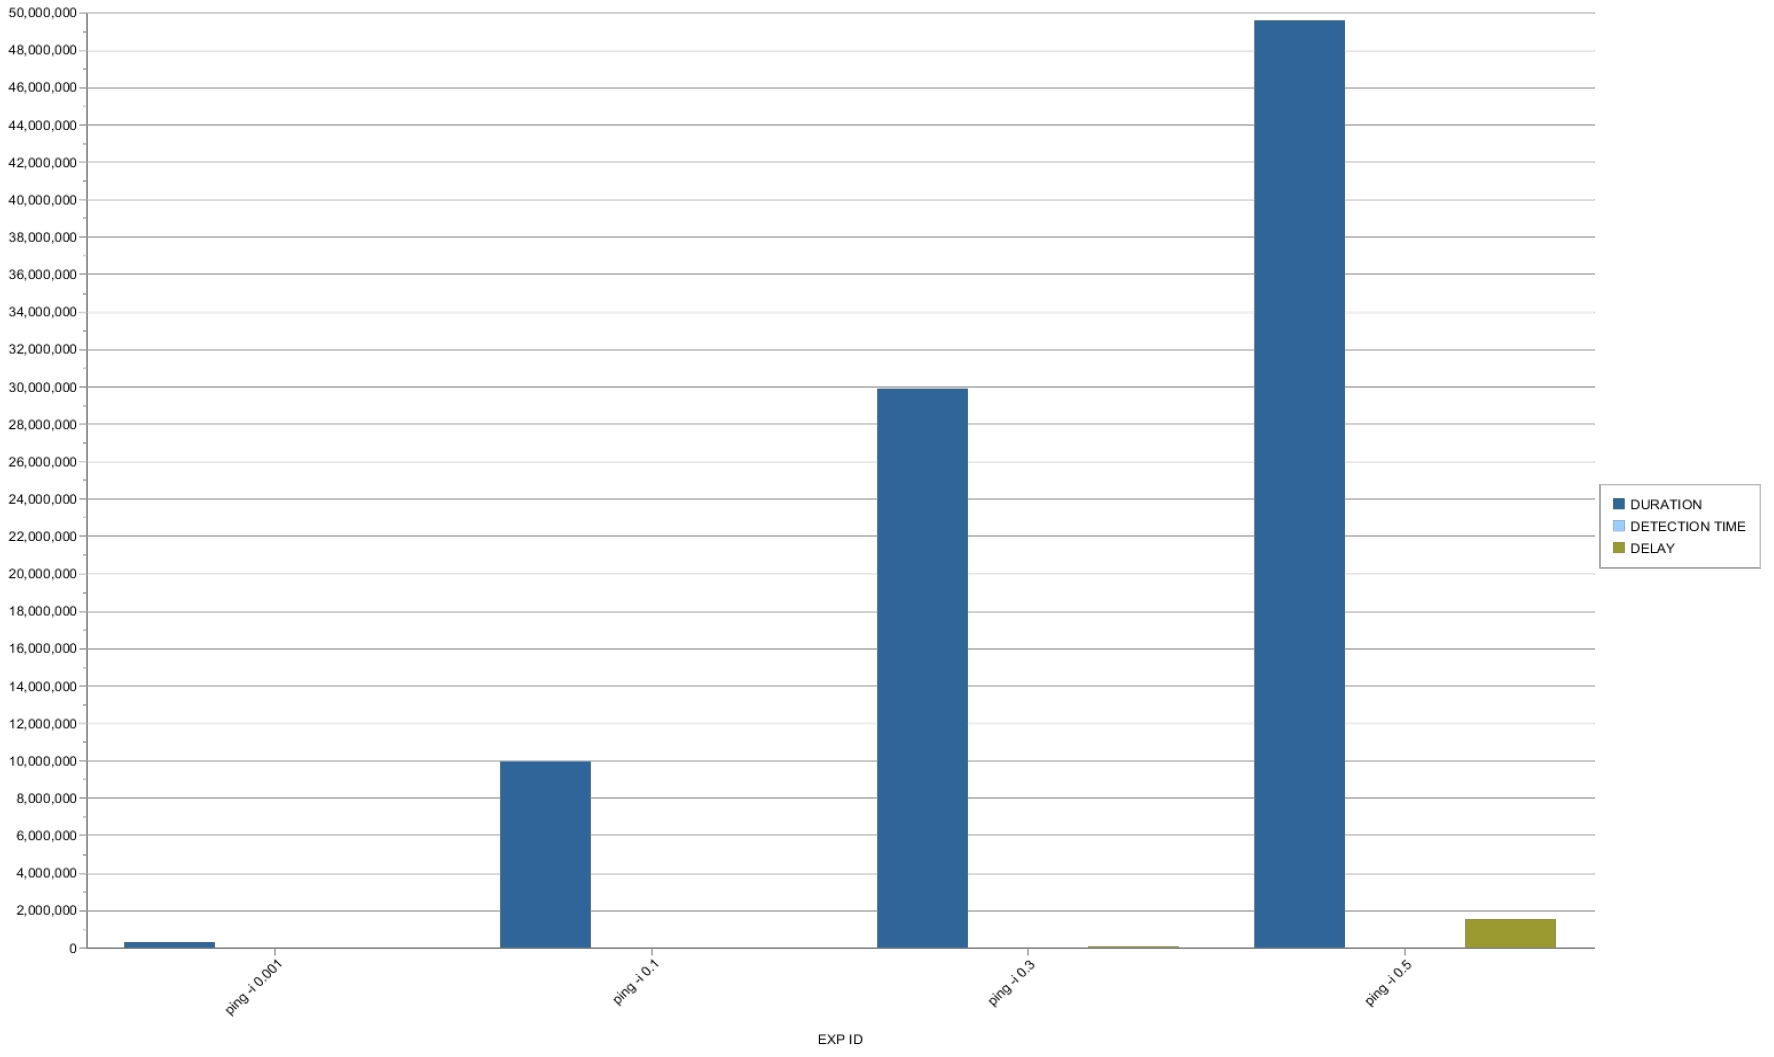
\includegraphics[scale=0.3]{figure/tempi_ping.jpg}\\

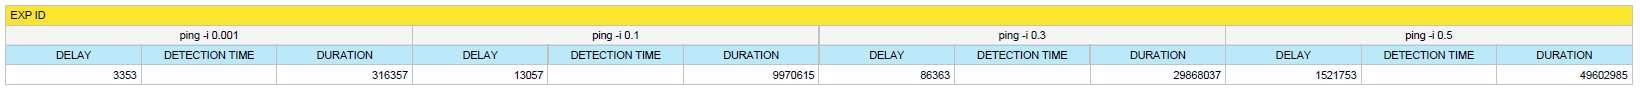
\includegraphics[scale=0.3]{figure/tabella_ping.jpg}


